\documentclass{beamer}
\beamertemplatenavigationsymbolsempty
\usecolortheme{beaver}
\setbeamertemplate{blocks}[rounded=true, shadow=true]
\setbeamertemplate{footline}[page number]
%
\usepackage{cmap}
\usepackage[utf8]{inputenc}
\usepackage[english, russian]{babel}
\usepackage{amssymb,amsfonts,amsmath,mathtext}
\usepackage{subfig}
\usepackage[all]{xy}
\usepackage{array}
\usepackage{multicol}
\usepackage{hyperref}
\usepackage{hhline}
\usepackage{algorithmic}
\usepackage{algorithm}

\usepackage[backend=bibtex, style=authoryear]{biblatex}
\bibliography{Slides}

\usepackage{mathtools}
\DeclarePairedDelimiterX{\infdivx}[2]{(}{)}{#1\;\delimsize\|\;#2}
%----------------------------------------------------------------------------------------------------------
\title[\hbox to 56mm{Bandits}]{ Бандиты в Query Selection }
\author[В.\,П. Шестаков]{Шестаков Владимир Павлович}
\institute{Московский физико-технический институт}
\date{\footnotesize
\par\smallskip\emph{Курс:} Автоматизация научных исследований
\par\smallskip\emph{Эксперт:} Ю.\,В.~Дорн
\par\smallskip\emph{Консультант:} И.\,М.~Латыпов
\par\bigskip\small 2025}
%----------------------------------------------------------------------------------------------------------
\begin{document}
%----------------------------------------------------------------------------------------------------------
\begin{frame}
\thispagestyle{empty}
\maketitle
\end{frame}
%-----------------------------------------------------------------------------------------------------
\begin{frame}{Задача и цель исследования}

\begin{block}{Задача}
  Воспроизвести результаты алгоритма Bao, модифицировать его различныи способами и проверить
\end{block}
\begin{block}{Цель}
  Исследовать влияние изменений алгоритма на качество
\end{block}

\end{frame}
%----------------------------------------------------------------------------------------------------------
\begin{frame}{Литература}
\nocite{bao}
\nocite{bandit-intro}
\printbibliography
\end{frame}
%----------------------------------------------------------------------------------------------------------
\begin{frame}{Начальная проблема: Query Optimization}
\begin{enumerate}
    \item
		Рост данных приводит к замедлению исполнения SELECT запросов

  \item
    Решение: оптимизаторы запросов. Два вида оптимизаторов: статические и динамически изменяемые
    \end{enumerate}

\begin{columns}[T]
\column{0.5\textwidth}
\begin{center}
\includegraphics[width=5cm]{query-optimizer-structure.png}
\end{center}
\column{0.5\textwidth}
\includegraphics[width=5cm]{query-plane-tree.png}
\end{columns}

\end{frame}
%-----------------------------------------------------------------------------------------------------
\begin{frame}{Алгоритм Bao}
\begin{center}
\includegraphics[width=8cm]{bao.png}
\end{center}
\end{frame}
%----------------------------------------------------------------------------------------------------------
\begin{frame}{Первые результаты}

\begin{columns}[T]
\column{0.5\textwidth}
\begin{center}
\includegraphics[width=5cm]{article-results.png}
\end{center}
\column{0.5\textwidth}
\begin{center}
\includegraphics[width=5cm]{real-results.png}
\end{center}
\end{columns}

\end{frame}
%----------------------------------------------------------------------------------------------------------
\begin{frame}{Дальнейшие эксперименты}
\begin{center}
\includegraphics[width=10cm]{diff-algos.png}
\end{center}
\end{frame}
%----------------------------------------------------------------------------------------------------------
\begin{frame}{График CDF}
\begin{center}
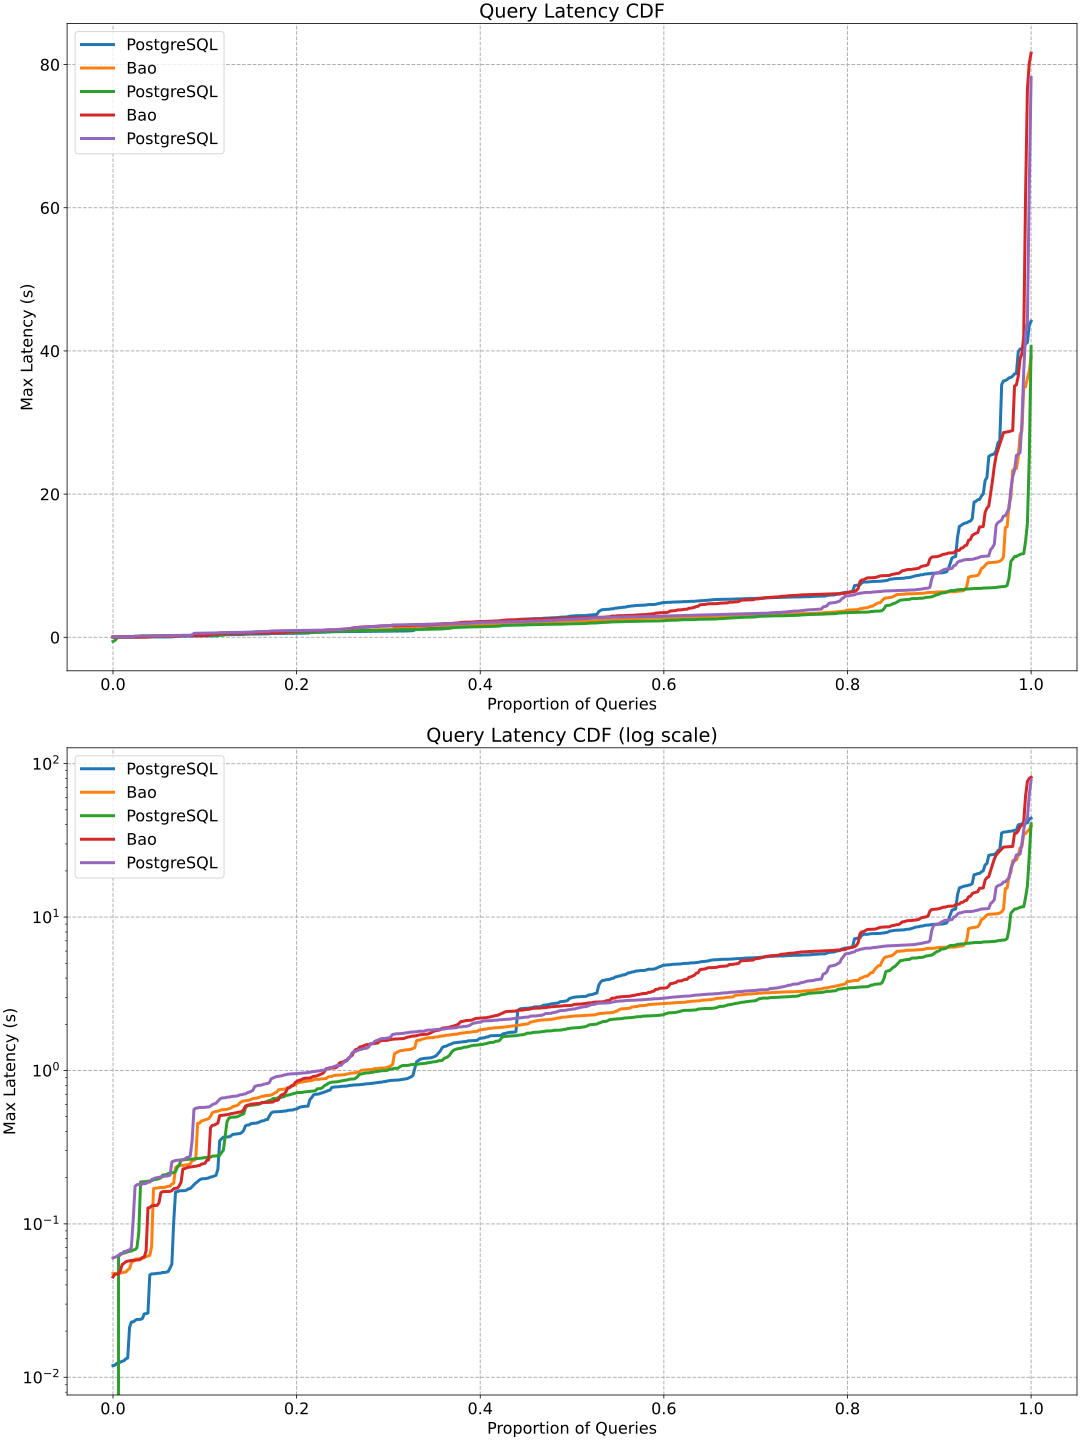
\includegraphics[width=10cm]{cdf.jpg}
\end{center}
\end{frame}
%----------------------------------------------------------------------------------------------------------
\begin{frame}{Таблица сравнения результатов экспериментов по некоторым запросам}
\begin{center}
\includegraphics[width=10cm]{table.jpg}
\end{center}
\end{frame}

%----------------------------------------------------------------------------------------------------------
\begin{frame}{Заключение}
  \begin{itemize}
      \item Получены результаты работы модификаций алгоритмов
      \item Некоторые из модификаций лучше изначального алгоритма по определённым качествам
      \item Есть потенциал дальнейшего улучшения
  \end{itemize}
\end{frame}
%----------------------------------------------------------------------------------------------------------
\end{document} 